\documentclass[12pt,a4paper]{article}
\title{MATH1110 Lec 009 Week 6-F}
\author{Benjamin Thompson}
\date{October 1, 2021}

\newcommand{\vspaceC}{\vspace{4cm}}
\usepackage[left=2cm,right=2cm]{geometry}

\usepackage{tikz, tikz-3dplot}
\usetikzlibrary{arrows.meta,decorations.markings}
\usepackage{etoolbox}

\usepackage{pgfplots}

\pgfplotsset{every axis/.append style={
axis x line=middle,    % put the x axis in the middle
axis y line=middle,    % put the y axis in the middle
axis line style={-{Stealth[length=3mm]},color=black}, % arrows on the axis
minor tick num=1
}}

\usepackage{amsmath}
\usepackage{graphicx}

\usepackage{fancyhdr}
\pagestyle{fancy}

\fancyhf{}
\lhead{MATH1110 Sec 009}
\chead{Week 6-F}
\rhead{October 1, 2021}
\cfoot{}

\begin{document}
\subsection*{Quiz}
\begin{enumerate}
    \item Evaluate
    \[
        \lim_{\theta \rightarrow 0} \frac{\theta}{\tan \theta}
    \]
    if it exists. If it does not, explain why.
    \vspaceC
    \item The tangent to the curve $y = x^2$ at $x = 10$ intersects the $x$-axis. Find this intersection point.
    \vspaceC
    \item Let \[
    f(x) = \begin{cases}
        x + 1 & x < 0 \\
        1 - x^2 & x \geq 0. 
    \end{cases}
    \] Is $f$ differentiable at $x = 0$? Why / why not?
    \vspaceC
    \item Does $(pq)' = p'q'$ for all polynomials $p(x),q(x)?$ If not, give a pair of polynomials $(a(x),b(x))$ for which $(ab)' \ne a'b'$.
    \vspaceC
\newpage
\lhead{Name:}
    \item A polynomial $p(x)$, as well as its derivative $p'(x)$ and second derivative $p''(x)$ are plotted below. Match $p,p',p''$ with $A,B,C$.
\[
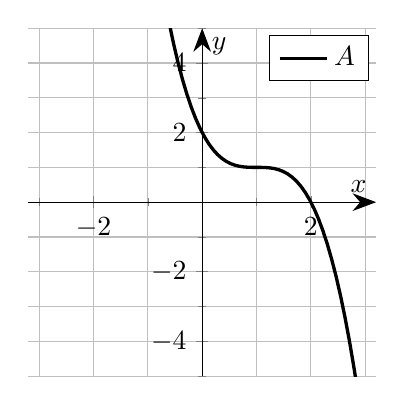
\begin{tikzpicture}
\begin{axis}[xlabel={$x$},ylabel={$y$},width=6cm, height=6cm, xmin=-3.2,xmax=3.2, ymin=-5,ymax=5, grid=both]
\addplot [very thick, domain=-4:4,samples=100]{-1*(x-1)^3 + 1};
\addlegendentry{$A$}
\end{axis}
\end{tikzpicture}
\quad
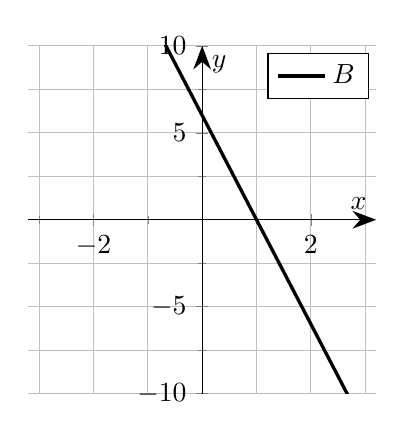
\begin{tikzpicture}
\begin{axis}[xlabel={$x$},ylabel={$y$},width=6cm, height=6cm, xmin=-3.2,xmax=3.2, ymin=-10,ymax=10, grid=both]
\addplot [very thick, domain=-4:4,samples=100]{-6*(x-1)};
\addlegendentry{$B$}
\end{axis}
\end{tikzpicture}
\quad
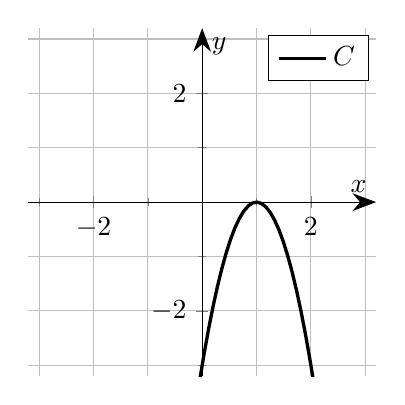
\begin{tikzpicture}
\begin{axis}[xlabel={$x$},ylabel={$y$},width=6cm, height=6cm, xmin=-3.2,xmax=3.2, ymin=-3.2,ymax=3.2, grid=both]
\addplot [very thick, domain=-4:4,samples=100]{-3*(x-1)^2};
\addlegendentry{$C$}
\end{axis}
\end{tikzpicture}
\]
\end{enumerate}

\end{document}
